% \appendix
\addtocontents{toc}{\protect\setcounter{tocdepth}{0}}

\renewcommand{\thechapter}{A}
\chapter{Appendix}

\section{GradCAM++ Importance Weights}\label{sec:grad-cam-plus-plus-weight-derivation}

Without the loss of generality, let us fix unit $k$ with the highest activation $A^k_{ij}$.
Since we utilize the GMP layer, all partial derivatives in \myref{Equation}{eq:grad-cam-pp-weights} will be zero, except for the one corresponding to the highest activation.
As a result, we can dismiss both sums, and the partial derivative weight becomes 
\begin{equation}
    i_{ck} = \alpha^{ck}_{ij} \relu(\frac{\partial Y^c}{\partial A^k_{ij}}).
\end{equation}
Authors already derived the activated score $Y^c = \exp(y^c)$ for us, and given the architecture of our model, the following set of equations holds:
\begin{equation}
\begin{aligned}
  \frac{\partial Y^c}{\partial A_{ij}^k}       &= \exp(y^c) \frac{\partial y^c}{\partial A_{ij}^k}     &&= \exp(y^c) w_{ck}     \\
  \frac{\partial^2 Y^c}{\partial (A_{ij}^k)^2} &= \exp(y^c) \bigl(\frac{\partial y^c}{\partial A_{ij}^k}\bigr)^2 &&= \exp(y^c) (w_{ck})^2 \\
  \frac{\partial^3 Y^c}{\partial (A_{ij}^k)^3} &= \exp(y^c) \bigl(\frac{\partial y^c}{\partial A_{ij}^k}\bigr)^3 &&= \exp(y^c) (w_{ck})^3.
\end{aligned}
\end{equation}

Plugging it all together, we get 
\begin{equation}
    \alpha_{ij}^{ck} = \frac{\exp(y^c) (w_{ck})^2}{2 \exp(y^c) (w_{ck})^2 + A^k_{ij} \exp(y^c) (w_{ck})^3} = \frac{1}{2 + A^k_{ij}w_{ck}}
\end{equation}
and subsequently
\begin{equation}
    i_{ck} = \frac{1}{2 + A^k_{ij}w_{ck}} \relu\bigr(\exp(y^c)w_{ck}\bigl).
\end{equation}

\pagebreak

\section{Convolutional Versus Pooling Layer for CAM-Based Methods}\label{sec:conv-vs-pool}

While it may seem natural to compute the saliency maps for the last convolutional layer, we decided to explore our options.

The final convolutional layer produces $512$ activation maps, each containing $32 \times 32$ activations.
If we upsample the weighted activation map $A^k$ to the size of $512 \times 512$ pixels, each spatial activation corresponds to a $16 \times 16$ part of the upsampled activation map.
If we use the last pooling layer instead, the dimensions are reversed, and individual elements of $16 \times 16$ pooled activation map will correspond to $32 \times 32$ pixels in the upsampled saliency map.
The production setting for Occlusion uses a patch of $55 \times 55$ pixels, with $27$ pixels stride.
We believe that the calculation of saliency maps for the pooled activations could closely resemble those produced by Occlusion.

While we have verified that saliency maps for the pooling layer are visually more similar to Occlusion than saliency maps for the convolutional layer, according to \cite{xai-anecdotal-evidence}, such an ``anecdotal'' conclusion is insufficient.
By applying the pooling operation, we condense the original activation map to $25$ percent of its original size, and this may lead to a loss of information when reconstructing the saliency map, undermining its faithfulness.
Thus, we conducted an additional experiment to compare both approaches using the faithfulness metric from \myref{Section}{sec:quant}.
The distribution of ROAD ratios is shown in \myref{Figure}{fig:road-conv-vs-pool}, and a visual comparison of both approaches is presented in \myref{Figure}{fig:conv-vs-pool}

Based on the results, we decided to continue with the saliency maps computed with respect to the pooling layer.
There is a negligible difference for CAM, and we posit the pooled saliency maps as more similar to Occlusion.
The same is true for HiResCAM; although the convolutional layer receives a much smaller ratio spread, the saliency maps tend to be more scattered and blurred.
For GradCAM++, using the convolutional layer is not an option.
Due to the inverse proportion between activation strength and the resulting importance weight, the less important regions are marked as more salient when the saliency map is computed for the last convolutional layer.
As we impute more of the area based on the saliency strength, the actual important regions are taken into account, and the model's score for perturbed images slowly decreases.
This is mostly tackled in the case of the pooling layer, as the more condensed activations seem to even out the indirect proportion. 
The difference for GradCAM++ regions imputed by the ROAD metric is shown in \myref{Figure}{fig:gradcampp-road-conv-vs-pool}.

\begin{figure}
    \begin{center}
    \begin{minipage}{1\textwidth}
      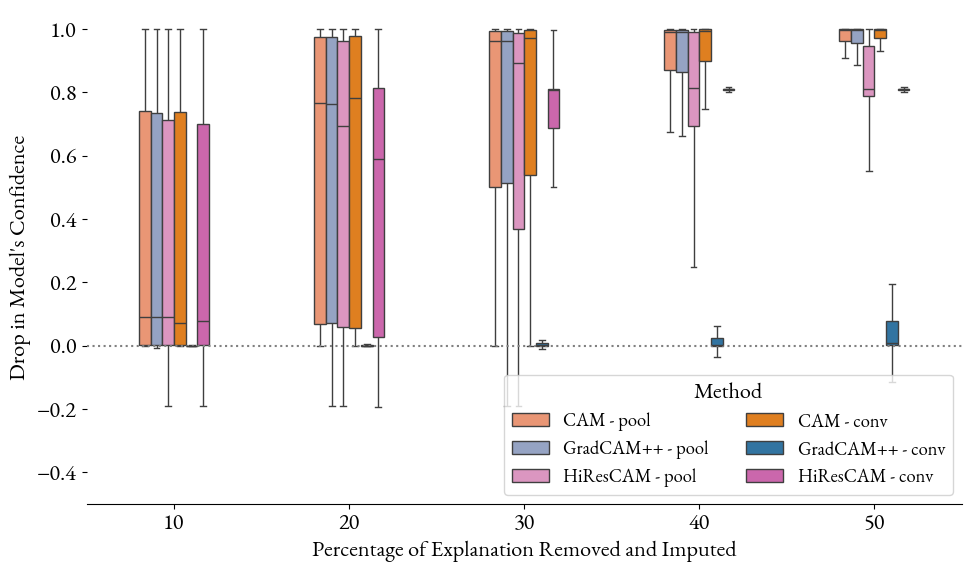
\includegraphics[width=\textwidth]{img/road-conv-vs-pool.png}
    \end{minipage}
    \caption{
    Comparison of ROAD ratios when attributing the last pooling versus the last convolutional layer.
    The CAM scores are almost the same, with the convolutional layer saliency maps being slightly more faithful according to our metric.
    HiResCAM achieves a significantly smaller spread when computing saliency maps with respect to the convolutional layer.
    However, the median is similar to its pooling layer counterpart.
    The largest difference comes for GradCAM++.
    We believe this is due to our finding in \myref{Subsection}{sub:gradcampp}, where activation strength is inversely proportional to the resulting importance weight.
    }
    \label{fig:road-conv-vs-pool}
    \end{center}
\end{figure}

\begin{figure}
    \begin{center}
    \begin{minipage}{0.5\textwidth}
      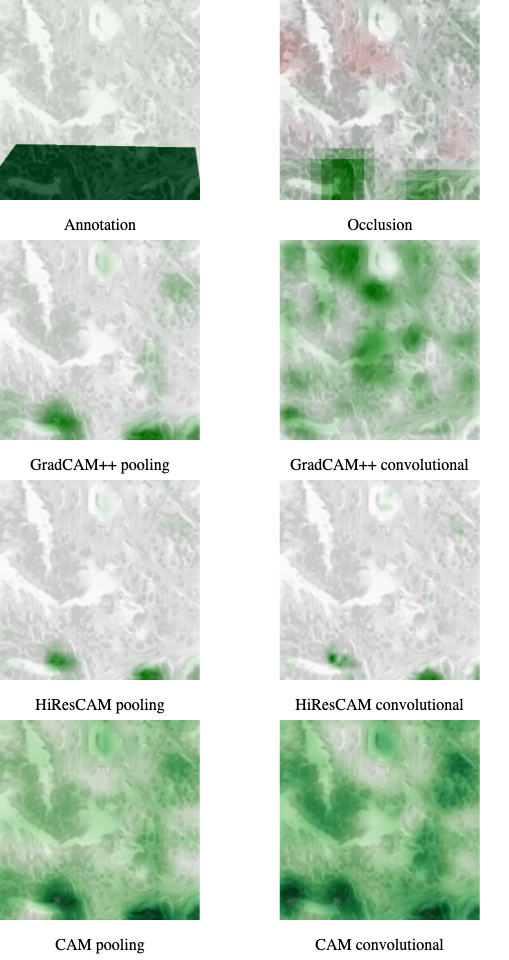
\includegraphics[width=\textwidth]{img/conv-vs-pool.png}
    \end{minipage}
    \caption{
    Visual comparison of saliency maps produced by CAM methods w.r.t. to the last pooling and the last convolutional layer of our model on a randomly selected tile.
    The underlying tile is shown in black and white to increase visual contrast.
    Note that Occlusion falls within the annotation boundaries, except for the top right corner.
    However, artifacts like this are removed using thresholding in the WSI browser.
    GradCAM++ is completely different when attributing the convolutional layer, focusing mostly on parts of the image that Occlusion and the annotation consider irrelevant.
    This changes once we compute the saliency maps w.r.t. the pooling layer.
    HiResCAM produces visually similar results, and despite producing similar results for this tile, the pooling saliency maps tend to cover larger and less scattered areas of the input tile.
    CAM is very liberal about the area covered, and the saliency maps are similar.
    However, the pooling one is easier to threshold because of the greater difference in saliency outside and inside the annotated area.
    }
    \label{fig:conv-vs-pool}
    \end{center}
\end{figure}

\begin{figure}
    \begin{center}
    \begin{minipage}{0.7\textwidth}
      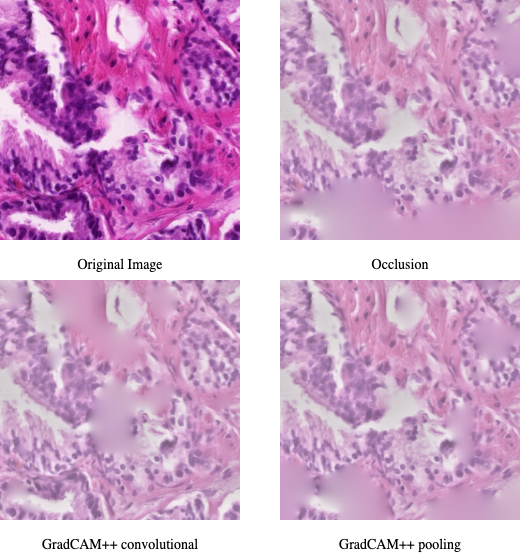
\includegraphics[width=\textwidth]{img/gradcampp-road-conv-vs-pool.png}
    \end{minipage}
    \caption{
    Visualization of different imputation results when we use the convolutional instead of the pooling layer for GradCAM++.
    On the original tile, the model accurately reports a confidence of $0.98$ for the presence of cancer.
    Both Occlusion and GradCAM++ w.r.t pooling layer accurately point to the relevant locations in the bottom of the tile, and the confidence on the perturbed tile drops to almost $0$.
    For GradCAM++ w.r.t. convolutional layer, the saliency map attributes different regions, and the confidence of our model on the perturbed image remains the same.
    We used \texttt{pytorch-grad-cam}'s implementation of visualizing the perturbed input, hence the discoloration.
    }
    \label{fig:gradcampp-road-conv-vs-pool}
    \end{center}
\end{figure}

\pagebreak

\section{Implementation}\label{sec:imple}

The source code of the benchmark, as well as the custom implementation of both CAM and HiResCAM, can be found in the \texttt{prostate-cancer} repository included in the supplementary materials. The source code is required to be run on the RationAI group's cluster, which has access to the test WSIs used for evaluation. Please visit the \texttt{README.md} file for installation and usage instructions. The \texttt{README.md} file also contains links to WSI with overlayed saliency maps available for inspection, given access rights issued by the RationAI group.
